\chapter{Methodology}

\section{Introduction}

Given the average driver's biological sensory capabilities, there are only have a few moments for them to react upon acknowledging the warning signals (e.g., lights and sirens) from \acrshort{EV}. The drivers must identify the \acrshort{EV}'s location and direction within these moments, understand their maneuver options, and safely execute their plan. However, it is common for primary urban roads to experience higher levels of service, ranging from steady traffic at high density (level D) to congestion (level F), as shown in figure ~\ref{fig:levels_of_service} \cite{archer_2005, traffic_data_computation_method_2018}. We define the rate of traffic service as the rate that vehicles pass a road section every hour. The following graph illustrates how the levels of service ratings are affected by the relationship between traffic volume, speed, and density. In the higher levels of service, maneuverability and speed are severely reduced, and high levels of vigilance are required to avoid accidents with neighbouring vehicles.

\begin{figure}
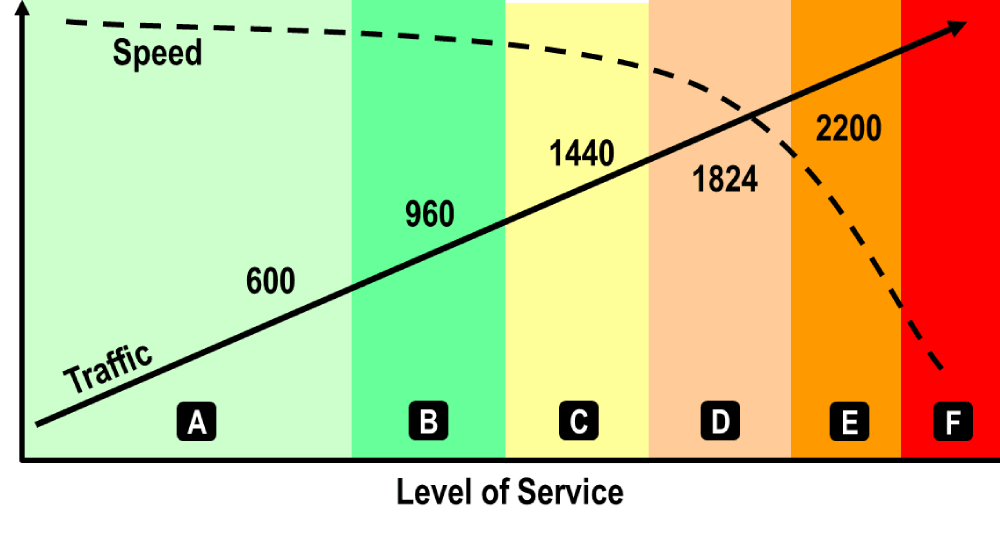
\includegraphics[width=\linewidth]{levels_of_service}
\caption{The relationship between traffic speed, density, volume, and the rating of Levels of Service.}
\label{fig:levels_of_service}
\end{figure}

!\cite{Untitled}(https://s3-us-west-2.amazonaws.com/secure.notion-static.com/152bf75f-1920-4a6a-81e5-791d3de665c7/Untitled.png)

Source: [https://transportgeography.org/contents/methods/transport-technical-economic-performance-indicators/levels-of-service-road-transportation/](https://transportgeography.org/contents/methods/transport-technical-economic-performance-indicators/levels-of-service-road-transportation/)

In situations of higher levels of service, drivers are therefore unable to react effectively to emergency signals, as they lack the space, speed, and visibility to clear a path, ultimately slowing or even preventing the \acrshort{EV} from traversing their route, which may have fatal ramifications \cite{Hsiao2018, Buchenscheit2009, Vlad2008, Sukru2020}.

However, given that traffic congestion is a non-linear function, studies show that even a small reduction in traffic volume can cause a proportionally larger reduction in delays [[https://transportgeography.org/contents/methods/transport-technical-economic-performance-indicators/levels-of-service-road-transportation/](https://transportgeography.org/contents/methods/transport-technical-economic-performance-indicators/levels-of-service-road-transportation/)] {TODO: finish citation}. Therefore, we aim to reduce the traffic volume along the paths of \acrshort{EV} by guiding selected CVs onto non-primary roads just in time to avoid conflicts with \acrshort{EV}.

This approach minimizes the risk of collision and delays as the levels of service for the primary roads will enter lower ratings, creating a calmer environment with more space and time to react to emergency signals. To achieve this reduction in the levels of service, we created an \acrshort{ITS} (Intelligent Transporation System) that autonomously mediates traffic volume between primary and second roads during emergencies. This chapter will outline the rationale behind the road network designs, scenario designs, software designs, the simulation setup, and the process of data collection.

\section{Research Design}

Our \acrshort{ITS} system comprises two main components: a (1) cloud-based server and a (2) \acrshort{OBU}. For proof of concept, we simulate emergency traffic scenarios that test \acrshort{EV}'s and civilian drivers' safety performance against varying penetration rates of \acrshort{OBU}-equipped vehicles.

Due to time constraints upon this research and the various programming languages involved, the implementation of the server component will be Google Cloud Platform (GCP)'s Cloud Function services. This architecture creates a language-agnostic solution that simplifies the communication between all the modules needed to control the simulation and the decision-making.

We use the open-source simulation software \cite{SUMO}(https://sumo.dlr.de/docs/index.html) (\textbf{S}imulation of \textbf{U}rban \textbf{MO}bility) to design, build, and conduct our urban traffic scenarios outlined in this chapter. We also use and build upon various tools provided by SUMO to create custom vehicle types and reproducible simulations. The custom supporting scripts and files required to reproduce our research are available on Github: https://github.com/DFazekas/thesis_simulation.

SUMO provides a TCP-based client/server module called TraCI (Traffic Control Interface). This module enables the control and modification of the simulation via a server. 

\begin{figure}
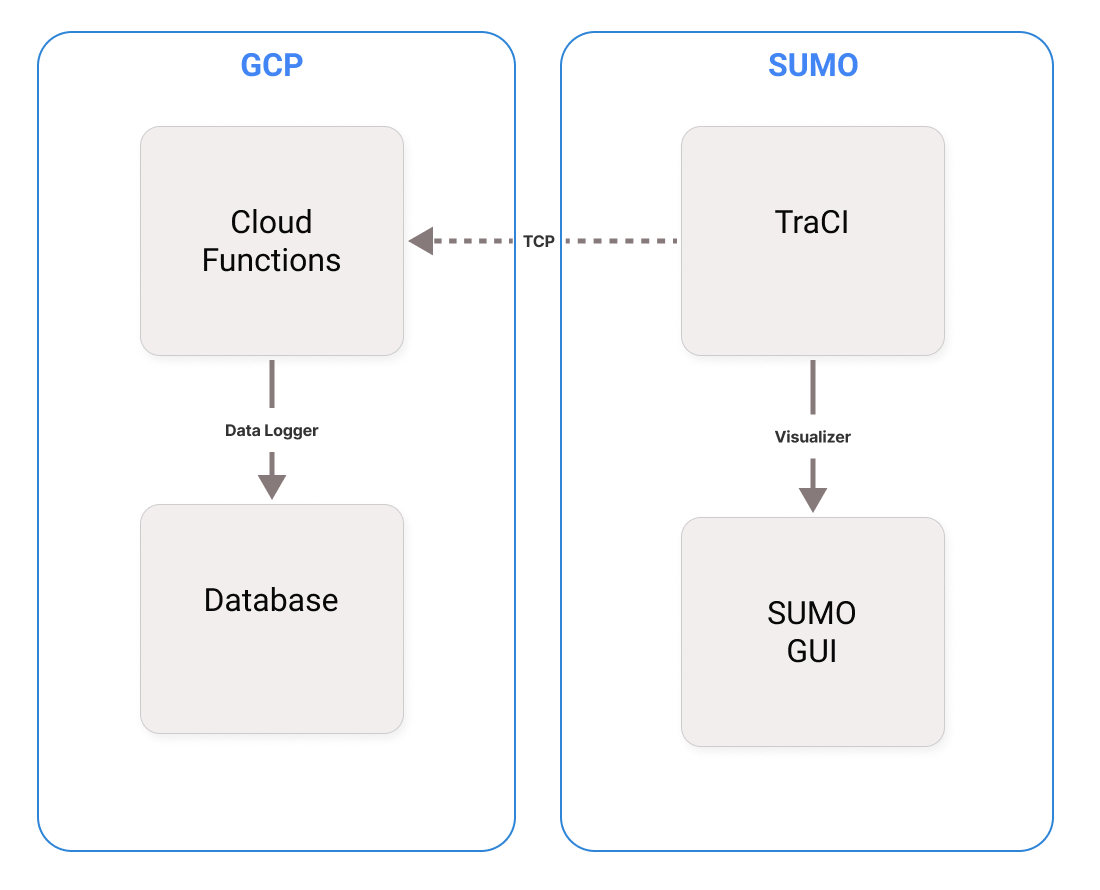
\includegraphics[width=\linewidth]{integration_architecture_overview}
\caption{A Communication Overview of SUMO and GCP Cloud Services.}
\label{fig:integration_architecture_overview}
\end{figure}

![integration_architecture_overview.jpeg](https://s3-us-west-2.amazonaws.com/secure.notion-static.com/1eb53637-2cf3-4495-84e1-86f9edeafdc8/integration_architecture_overview.jpeg)

Figure: integration_architecture_overview

Figure ~\ref{fig:integration_architecture_overview} depicts a high-level overview of how TraCI enables the communication between SUMO and GCP services. In this chapter, we will examine and elaborate on how to set up each segment of this figure.

\subsection{Cloud Functions}

\subsection{Cloud Database}

\subsection{SUMO TraCI}

\subsection{SUMO GUI}

\subsection{Road Network Design}

The SUMO software provides the opportunity to test the validity of our \acrshort{ITS} system against a plethora of variables and situations. The prospective benef\acrshort{its} of our \acrshort{ITS} system are proportional to the number of non-primary roads available within the geographical region under focus. For instance, the greater number of alternative roads and lanes that the \acrshort{ITS} system has at \acrshort{its} disposal, the greater impact it can have on alleviating traffic volume on primary roads. For these reasons, we will study the effectiveness of our \acrshort{ITS} system against multiple road network configurations.

A road network in SUMO comprises nodes (junctions) and edges (roads). Figure ~\ref{fig:single-lane_streets_and_junctions} depicts an example of a road network with nodes labelled arbitrarily as "N#" and edges as "L#". This example has two types of junctions: (1) default and (2) traffic lights. Default junctions have the minimum characteristics such as "right-of-way" and "approaching speed" rules, among others. Whereas traffic light junctions have additional characteristics that control traffic flow.

\begin{figure}
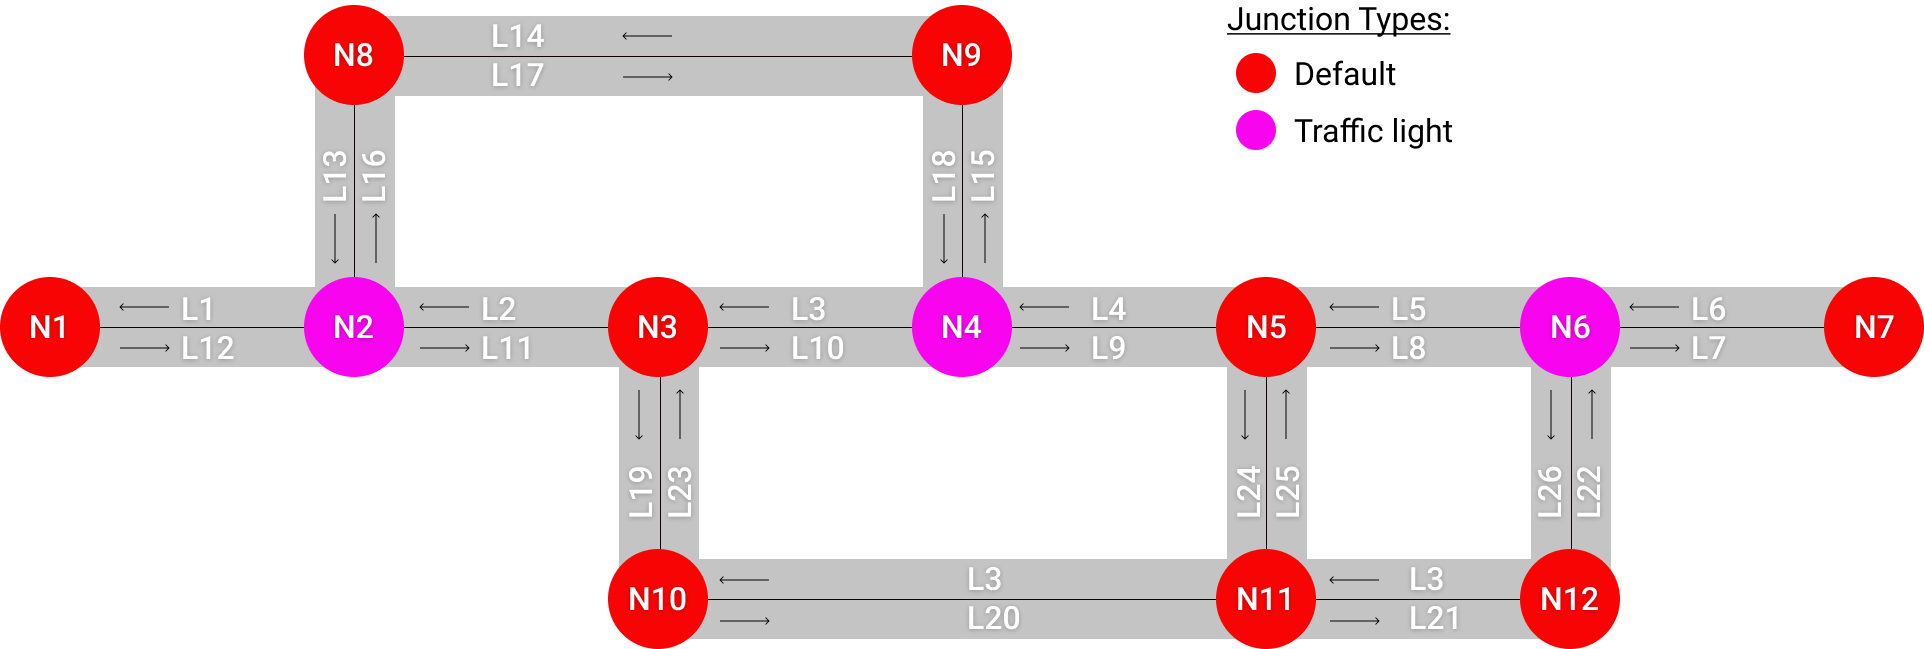
\includegraphics[width=\linewidth]{single-lane_streets_and_junctions}
\caption{A Single-Lane Road Network.}
\label{fig:single-lane_streets_and_junctions}
\end{figure}

![single_lane_streets_and_junctions.jpeg](https://s3-us-west-2.amazonaws.com/secure.notion-static.com/31751de9-5db9-4544-a75e-166cc46f0126/single_lane_streets_and_junctions.jpeg)

Figure: single-lane_streets_and_junctions.jpeg

One such alternative configuration to a road network includes increasing the number of lanes in either direction on an edge. Figure ~\ref{fig:multi-lane_streets_and_junctions} illustrates modifying the primary roads (i.e., N1 through N7) to include 2-lanes in both directions while keeping the secondary roads as single-lanes. These modifications enable the lane-changing behaviour of vehicles during emergencies, while also representing a more realistic urban road segment; it is uncommon for primary roads to be single-laned. 

\begin{figure}
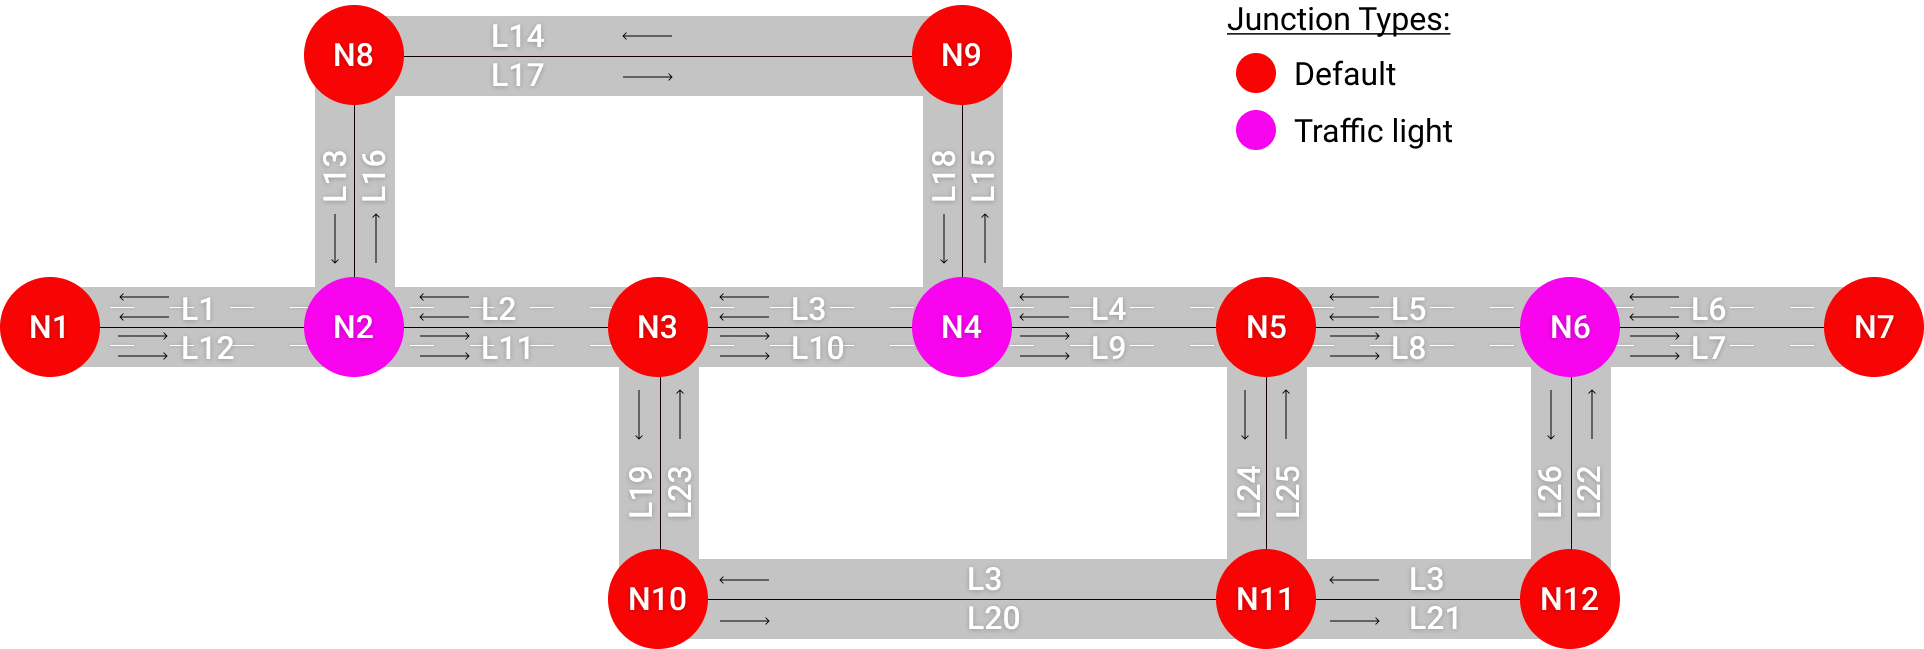
\includegraphics[width=\linewidth]{multi-lane_streets_and_junctions}
\caption{A Multi-Lane Road Network.}
\label{fig:multi-lane_streets_and_junctions}
\end{figure}

![multi-lane_streets_and_junctions.jpeg](https://s3-us-west-2.amazonaws.com/secure.notion-static.com/d8c055ba-1f04-41d1-8d0d-4450f2f106c6/multi-lane_streets_and_junctions.jpeg)

Figure: multi-lane_streets_and_junctions.jpeg

The following figures, ~\ref{fig:network_setup_junctions} and ~\ref{fig:network_setup_edges} show tabulation representations of Fig ~\ref{fig:single-lane_streets_and_junctions} that helps recreate the network using the Netedit tool provided by SUMO. 

Figure ~\ref{fig:network_setup_junctions} contains the details of each junction, from their type to their position. Although, it should be noted that Netedit does not use the term "Default" but instead uses "Unknown." The values in these columns can be set through Netedit via using the Inspect Tool and selecting an existing junction; \acrshort{its} attributes are displayed on the left panel, outlined in red in Fig ~\ref{fig:screenshot_netedit_junction_attributes}.

\begin{figure}
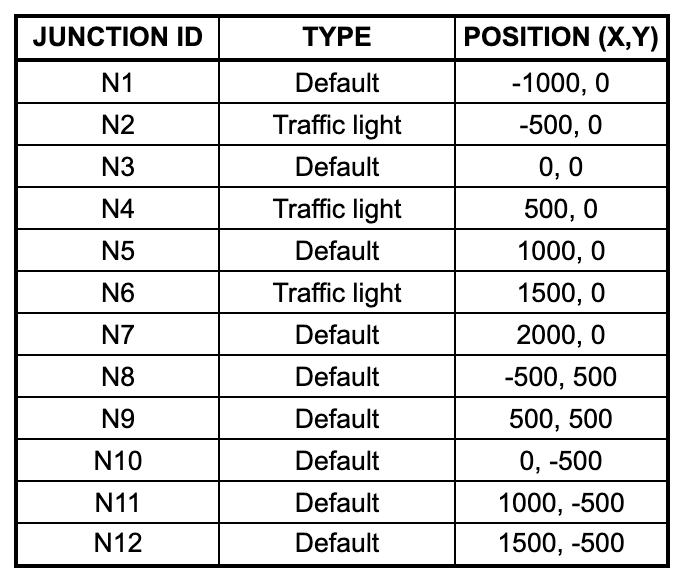
\includegraphics[width=\linewidth]{network_setup_junctions}
\caption{Table of Junctions: ID, Type, and Position.}
\label{fig:network_setup_junctions}
\end{figure}

![network_setup_junctions.jpeg](https://s3-us-west-2.amazonaws.com/secure.notion-static.com/68f5a3bb-65d6-4c99-878c-29c6ac66acc7/network_setup_junctions.jpeg)

Figure: network_setup_junctions

\begin{figure}
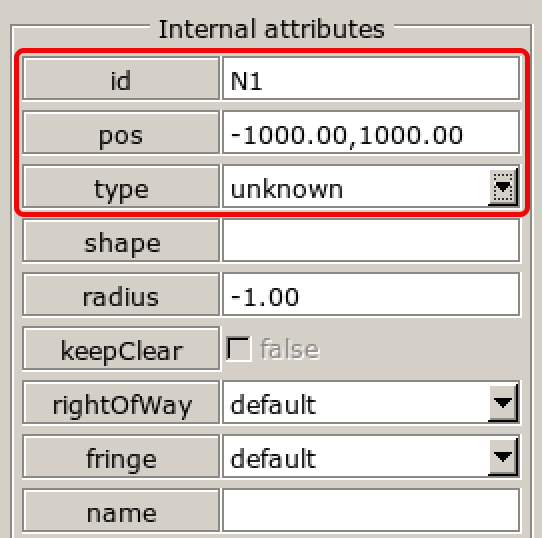
\includegraphics[width=\linewidth]{screenshot_netedit_junction_attributes}
\caption{Screenshot from Netedit: Junction Attributes.}
\label{fig:screenshot_netedit_junction_attributes}
\end{figure}

![screenshot_netedit_junction_attributes.jpeg](https://s3-us-west-2.amazonaws.com/secure.notion-static.com/e4036c1b-9fbe-494f-a201-b9376ebbcb6b/screenshot_netedit_junction_attributes.jpeg)

Figure: screenshot_netedit_junction_attributes

Figure ~\ref{fig:network_setup_edges} contains the information of each edge: their respective ID, the number of lanes, priority levels, and their origin and destination junction nodes. The number of lanes controls the available lanes per direction and enables vehicles to pass one another. Priority Levels control how important or preferred a lane is to drivers. The following screenshot (Figure ~\ref{fig:screenshot_netedit_edge_attributes}) outlines in red the corresponding attribute controls in Netedit after inspecting an edge.

\begin{figure}
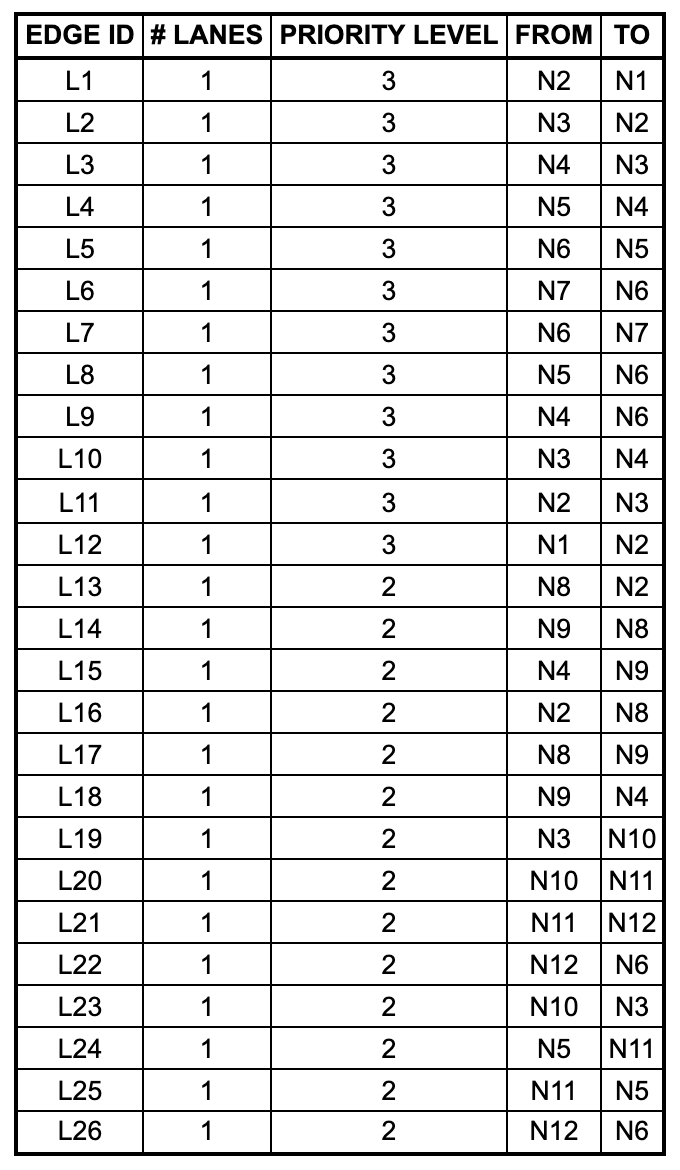
\includegraphics[width=\linewidth]{network_setup_edges}
\caption{Table of Edges: ID, # of Lanes, Priority Level, From Node, and To Node.}
\label{fig:network_setup_edges}
\end{figure}

![network_setup_edges.jpeg](https://s3-us-west-2.amazonaws.com/secure.notion-static.com/d253b830-b0d4-4972-b257-92b69c925f84/network_setup_edges.jpeg)

Figure: network_setup_edges

\begin{figure}
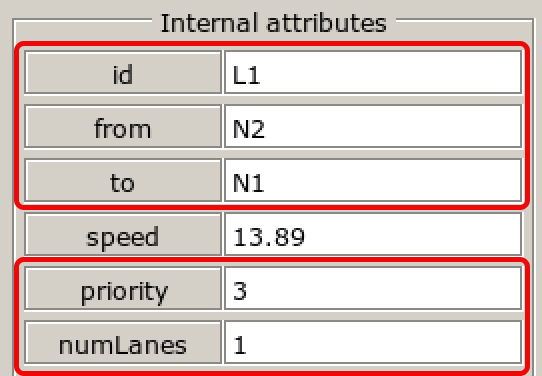
\includegraphics[width=\linewidth]{screenshot_netedit_edge_attributes}
\caption{Screenshot from Netedit: Edge Attributes.}
\label{fig:screenshot_netedit_edge_attributes}
\end{figure}

![screenshot_netedit_edge_attributes.jpeg](https://s3-us-west-2.amazonaws.com/secure.notion-static.com/165eccb6-c1dc-4c75-aa68-9779d96fd9e0/screenshot_netedit_edge_attributes.jpeg)

Figure: screenshot_netedit_edge_attributes

\subsection{Vehicle Models}

We designed four vehicular models, including (1) civilian vehicles, (2) connected civilian vehicles, (3) \acrshort{EV}, and (4) connected \acrshort{EV}. The models vary in behavioural properties, physical properties, and technological capabilities. For instance, we equip both connected civilian vehicles and connected \acrshort{EV} with devices enabling risk detection and communication with our cloud server. 

For instance, SSM devices log risks that the equipped vehicle encounters. We track multiple types of risks:

1. Time to Collision (TTC): where the following vehicle is faster than the leading vehicle.
2. SGAP: a measure of distance between bumpers (minus minGap) of the equipped vehicle and a leading vehicle.
3. TGAP: a time headway measured by spacing versus time between the equipped and leading vehicles.

The individual attributes for each type of vehicle model are shown in Figure ~\ref{fig:vehicle_models} and elaborated below:

![vehicle_models.jpeg](https://s3-us-west-2.amazonaws.com/secure.notion-static.com/291359b3-87b1-4232-953c-6cbd84977a72/vehicle_models.jpeg)

Figure: vehicle_models

\begin{figure}
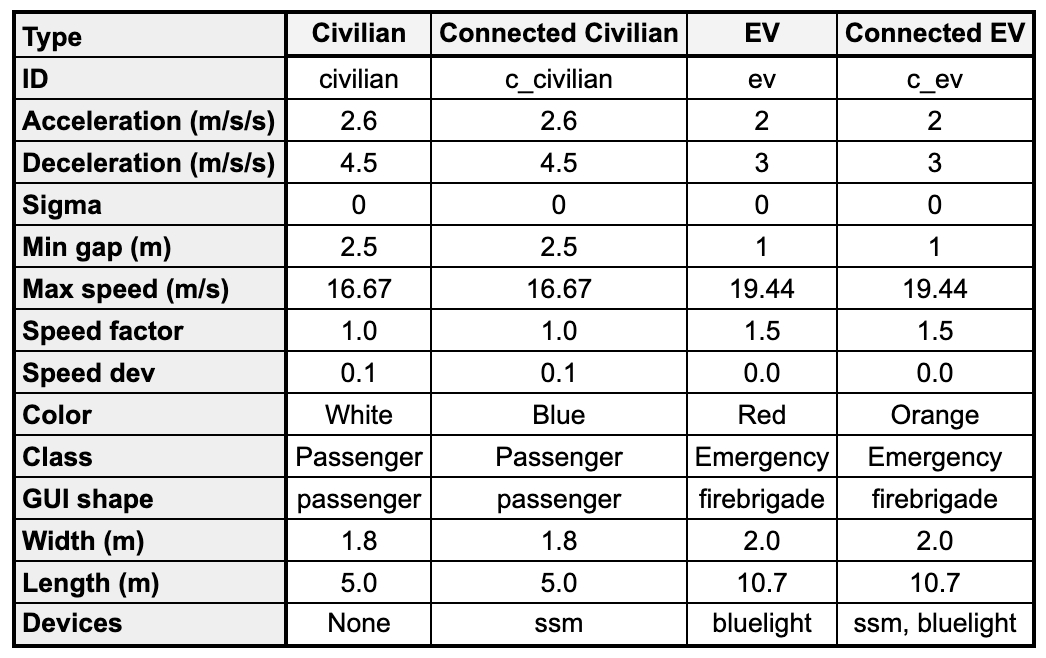
\includegraphics[width=\linewidth]{vehicle_models}
\caption{Table of Vehicle Models.}
\label{fig:vehicle_models}
\end{figure}

\textbf{Civilian Vehicle}

We designed the vehicles inheriting this model type to mimic an average white sedan. They have lengths and widths of 5.0 meters and 1.8 meters, respectfully. Capable of accelerating at 2.6 m/s/s and decelerating at 4.5 m/s/s with max speeds up to 16.67 m/s. These vehicles aim to keep a distance of 2.5 meters from leading vehicles.

\textbf{Connected Civilian Vehicle}

These CVs have almost the same attributes as a regular civilian vehicle, except their colour is blue, and they have an SSM device.

**Emergency Vehicle (\acrshort{EV})**

We chose red firetrucks as our base model for \acrshort{EV} as they are the largest and struggle the most at negotiating traffic. These vehicles are 10.7 meters in length and 2.0 meters in width. They can accelerate at 2.0 m/s/s and decelerate at 3.0 m/s/s. Although \acrshort{EV} are exempt by speed laws, they must still drive safely, and for that reason, we capped their max speed at 19.44 m/s, granting them a speed factor of 1.5 (i.e., 150\% of the posted road speed limit). These vehicles have Bluelight devices that simulate the "code-3-running" with emergency signals (i.e., lights and sirens), allowing them to exceed speed lim\acrshort{its}, run through red lights, and yield nearby traffic.

**Connected \acrshort{EV}**

These \acrshort{EV} have all the same attributes as above but are orange in colour and have an SSM and a Bluelight device.

\section{Data Collection Methods}

Both SUMO and the Cloud Functions report simulation data. Because SUMO uses the XML language for \acrshort{its} reporting and only generates data after a simulation completes, we configure SUMO to export locally. We later aggregate and process these local files into a single Cloud Database. The Cloud Functions, on the other hand, push directly to the Cloud Database during a simulation.

The data is broken into two parts:
\begin{enumerate}

\item Road-centric measurements for all vehicles passing through this segment include average speed, traffic flow, capacity, density, average time headway, total risk score, and events such as near collisions, congestion, and traffic signals.

\item Vehicular-centric measurements for each vehicle include speed, acceleration, path, delays, and frequencies of path modification and detected \acrshort{EV}.

\end{enumerate}
This list is not exhaustive and will be modified as the author grows familiar with the simulation software.

## Software & Technology Related Design

The SUMO simulator software manages the simulation component and offers various tools for importing data, designing models, designing networks, and tracking data. A running simulation will continuously measure and compute a wide range of road and vehicular-centric data.

The TraCI module is responsible for controlling the simulation and communicating with the Cloud Server. TraCI feeds the Cloud Functions data at a fixed interval throughout the running simulation and uses the response to make adjustments for select connected vehicles. The Cloud Functions evaluate localized risk assessment and perform decision-making such as slowing down, turning, and lane changing, as shown in the flowchart of Figure ~\ref{fig:vehicle_processing}.

The cloud server facilitates safer, smoother, and faster traffic for connected vehicles. The flowchart shown in Figure ~\ref{fig:server_processing} describes the relationship between the array of processes that this server is responsible for, including:
1. Path Generation
2. Prediction of ER Path Collision
3. Path Modification

![vehicle_processing.jpg](https://s3-us-west-2.amazonaws.com/secure.notion-static.com/64581c1c-c877-47bf-992e-ed1ed30de6e8/vehicle_processing.jpg)

Figure: vehicle_processing

\begin{figure}
\includegraphics[width=\linewidth]{vehicle_processing}
\caption{Flowchart of onboard vehicle processing.}
\label{fig:vehicle_processing}
\end{figure}

![server_processing.jpg](https://s3-us-west-2.amazonaws.com/secure.notion-static.com/6d5db242-1ece-4eb7-99b3-fb68960a8d74/server_processing.jpg)

Figure: server_processing

\\begin{figure}
	\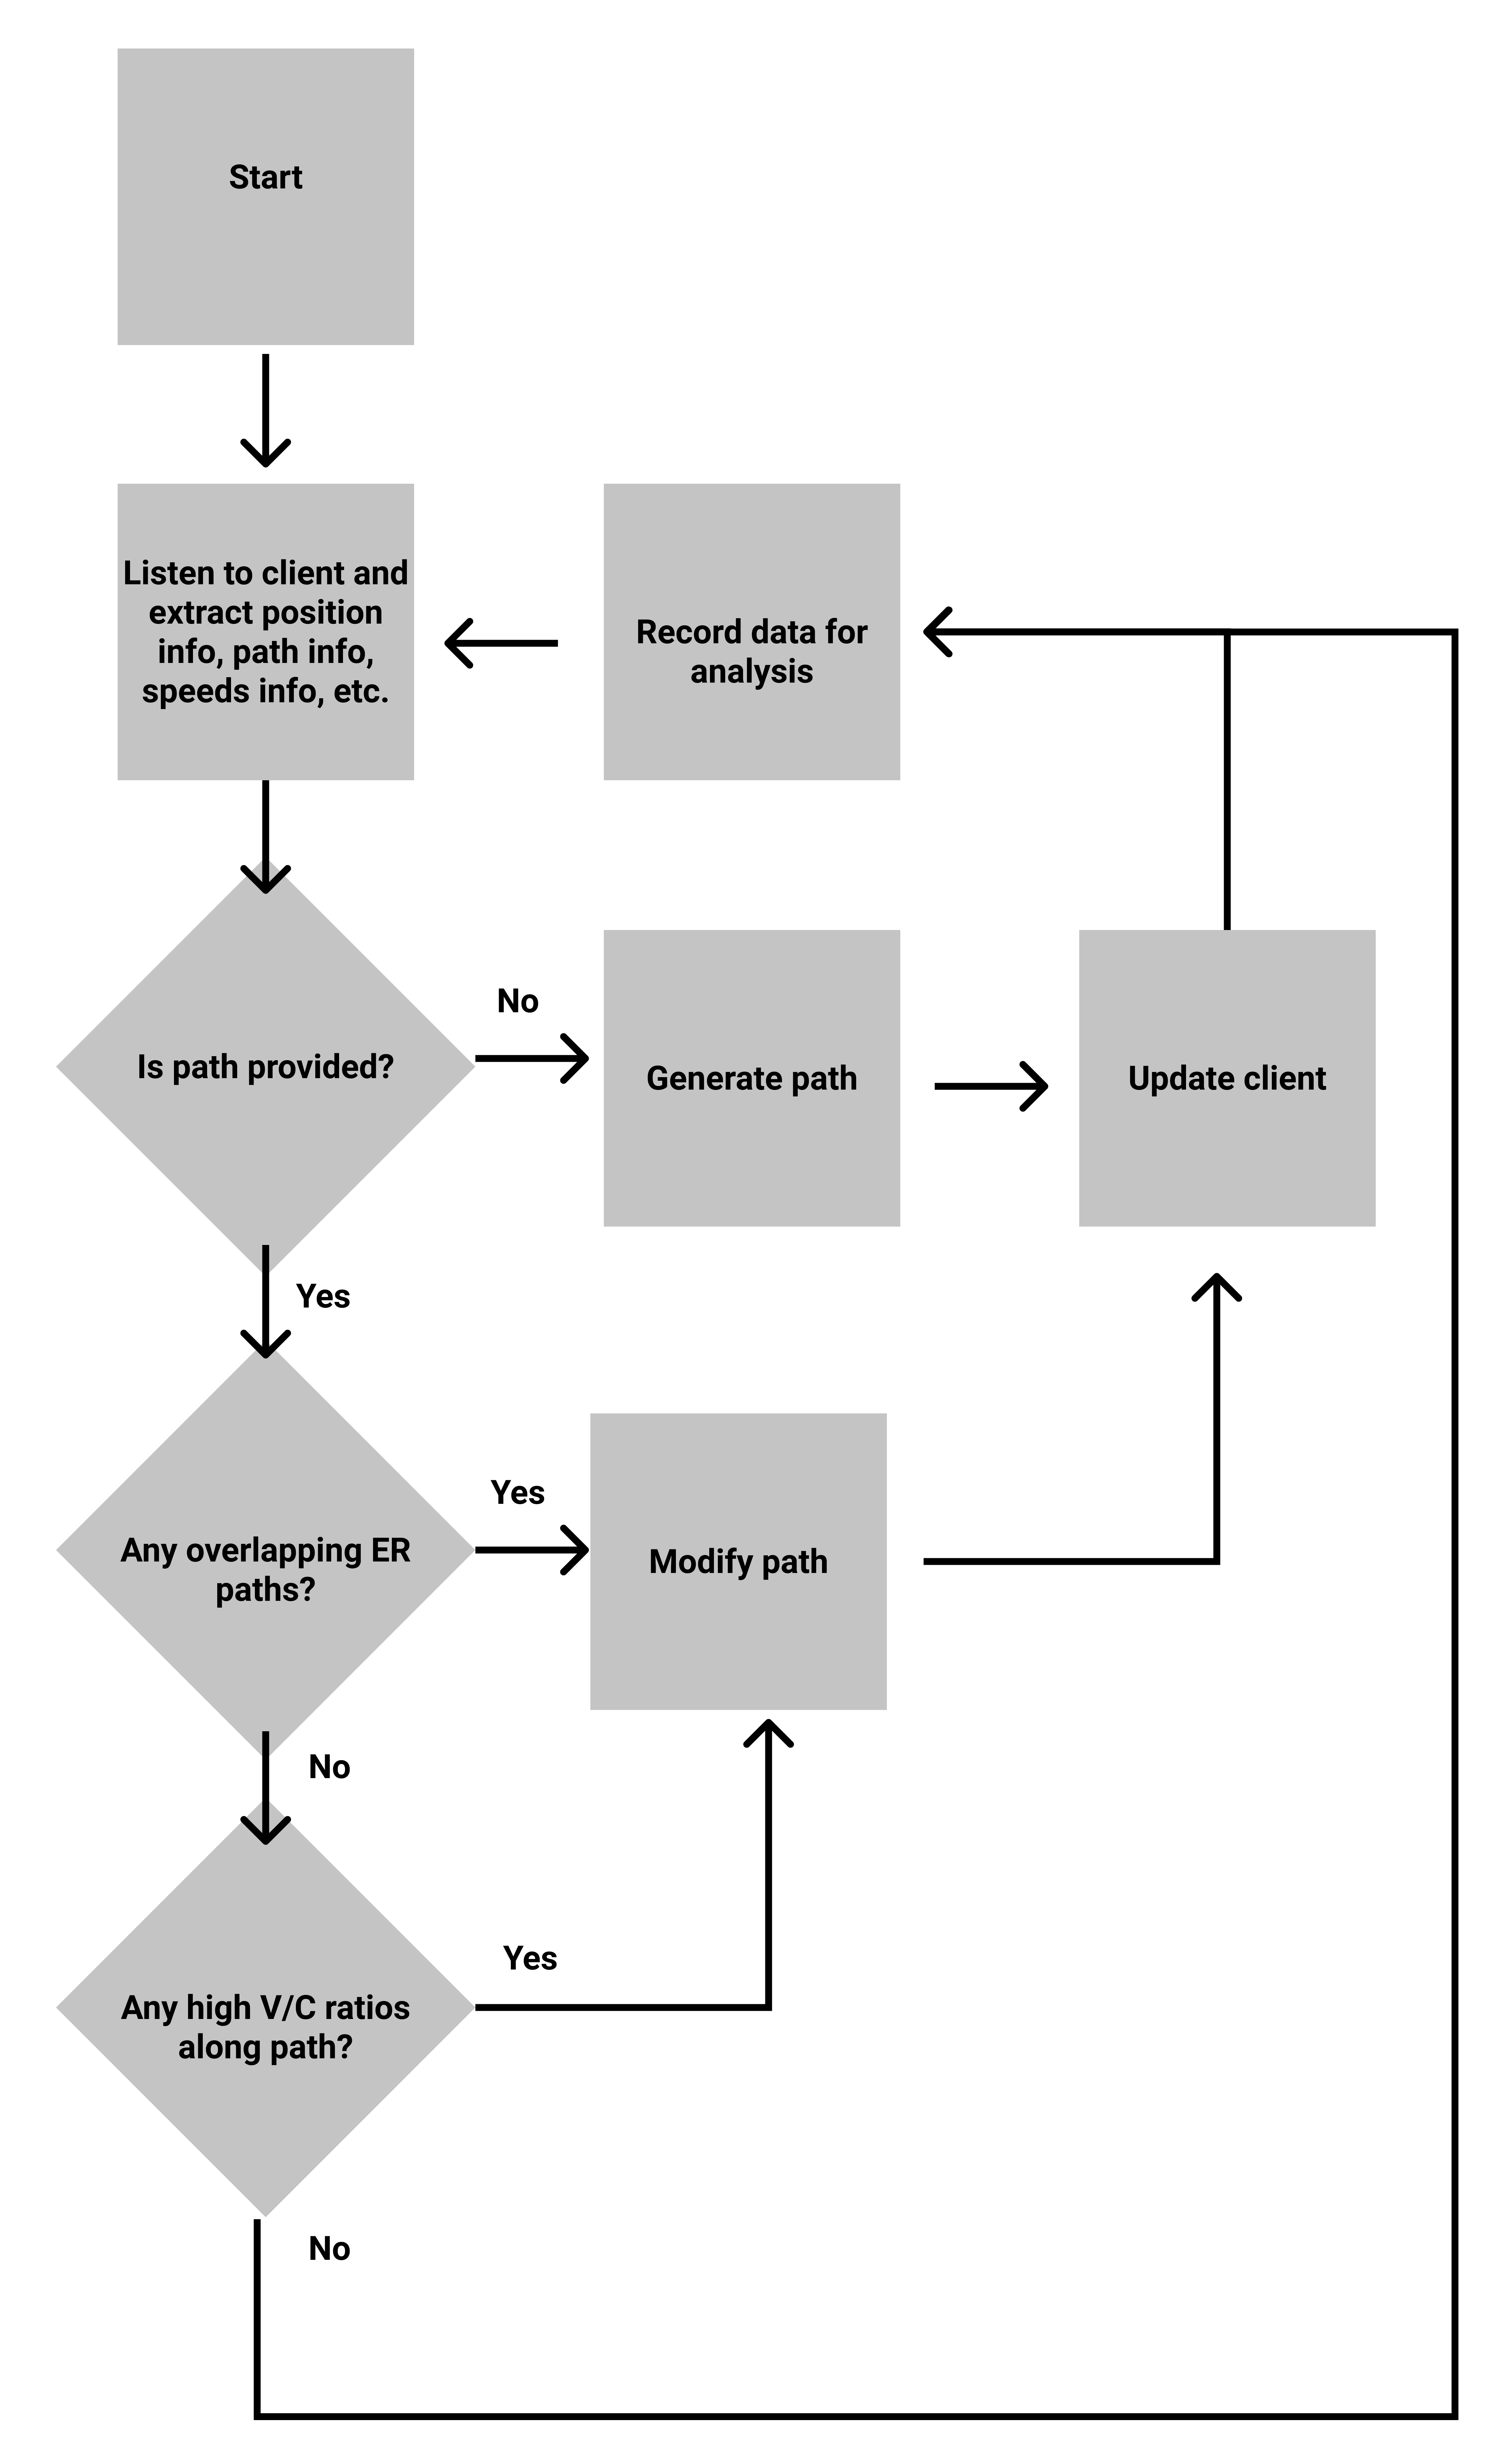
\includegraphics[width=\\linewidth]{server_processing}
	\\caption{Flowchart of cloud-based processing.}
	\\label{fig:server_processing}
\\end{figure}

\subsection{Path Generation}

This process is the first to be executed for every new CV initiating their commute. It considers the vehicle's current location, desired destination, and current traffic data to generate a path optimized for the lowest arrival time (i.e., fastest commute) using the <A* algorithm>. Figure ~\ref{fig:a-star_algorithm} depicts a minimalistic road segment with a path generated for an \acrshort{EV} between two points.

![a-star_algorithm.jpg](https://s3-us-west-2.amazonaws.com/secure.notion-static.com/bedb2952-c668-454a-92d1-319707765b1a/a-star_algorithm.jpg)

Figure: a-star_algorithm

\begin{figure}
\includegraphics[width=\linewidth]{a-star_algorithm}
\caption{Generated Path for an ER.}
\label{fig:a-star_algorithm}
\end{figure}

\subsection{Prediction of ER Path Collision}

This process predicts when and where a connected civilian vehicle might collide with an \acrshort{EV}. The pseudocode in Figure ~\ref{fig:algorithm_01_psuedocode} elaborates on detecting all possible collision points along the paths of these two vehicles, and Figure ~\ref{fig:algorithm_01_diagram} provides a visual demonstration.

![algorithm_01_psuedocode.jpg](https://s3-us-west-2.amazonaws.com/secure.notion-static.com/8245b95a-2eee-430a-9dee-c066890d41ec/algorithm_01_psuedocode.jpg)

Figure: algorithm_01_psuedocode

\begin{figure}
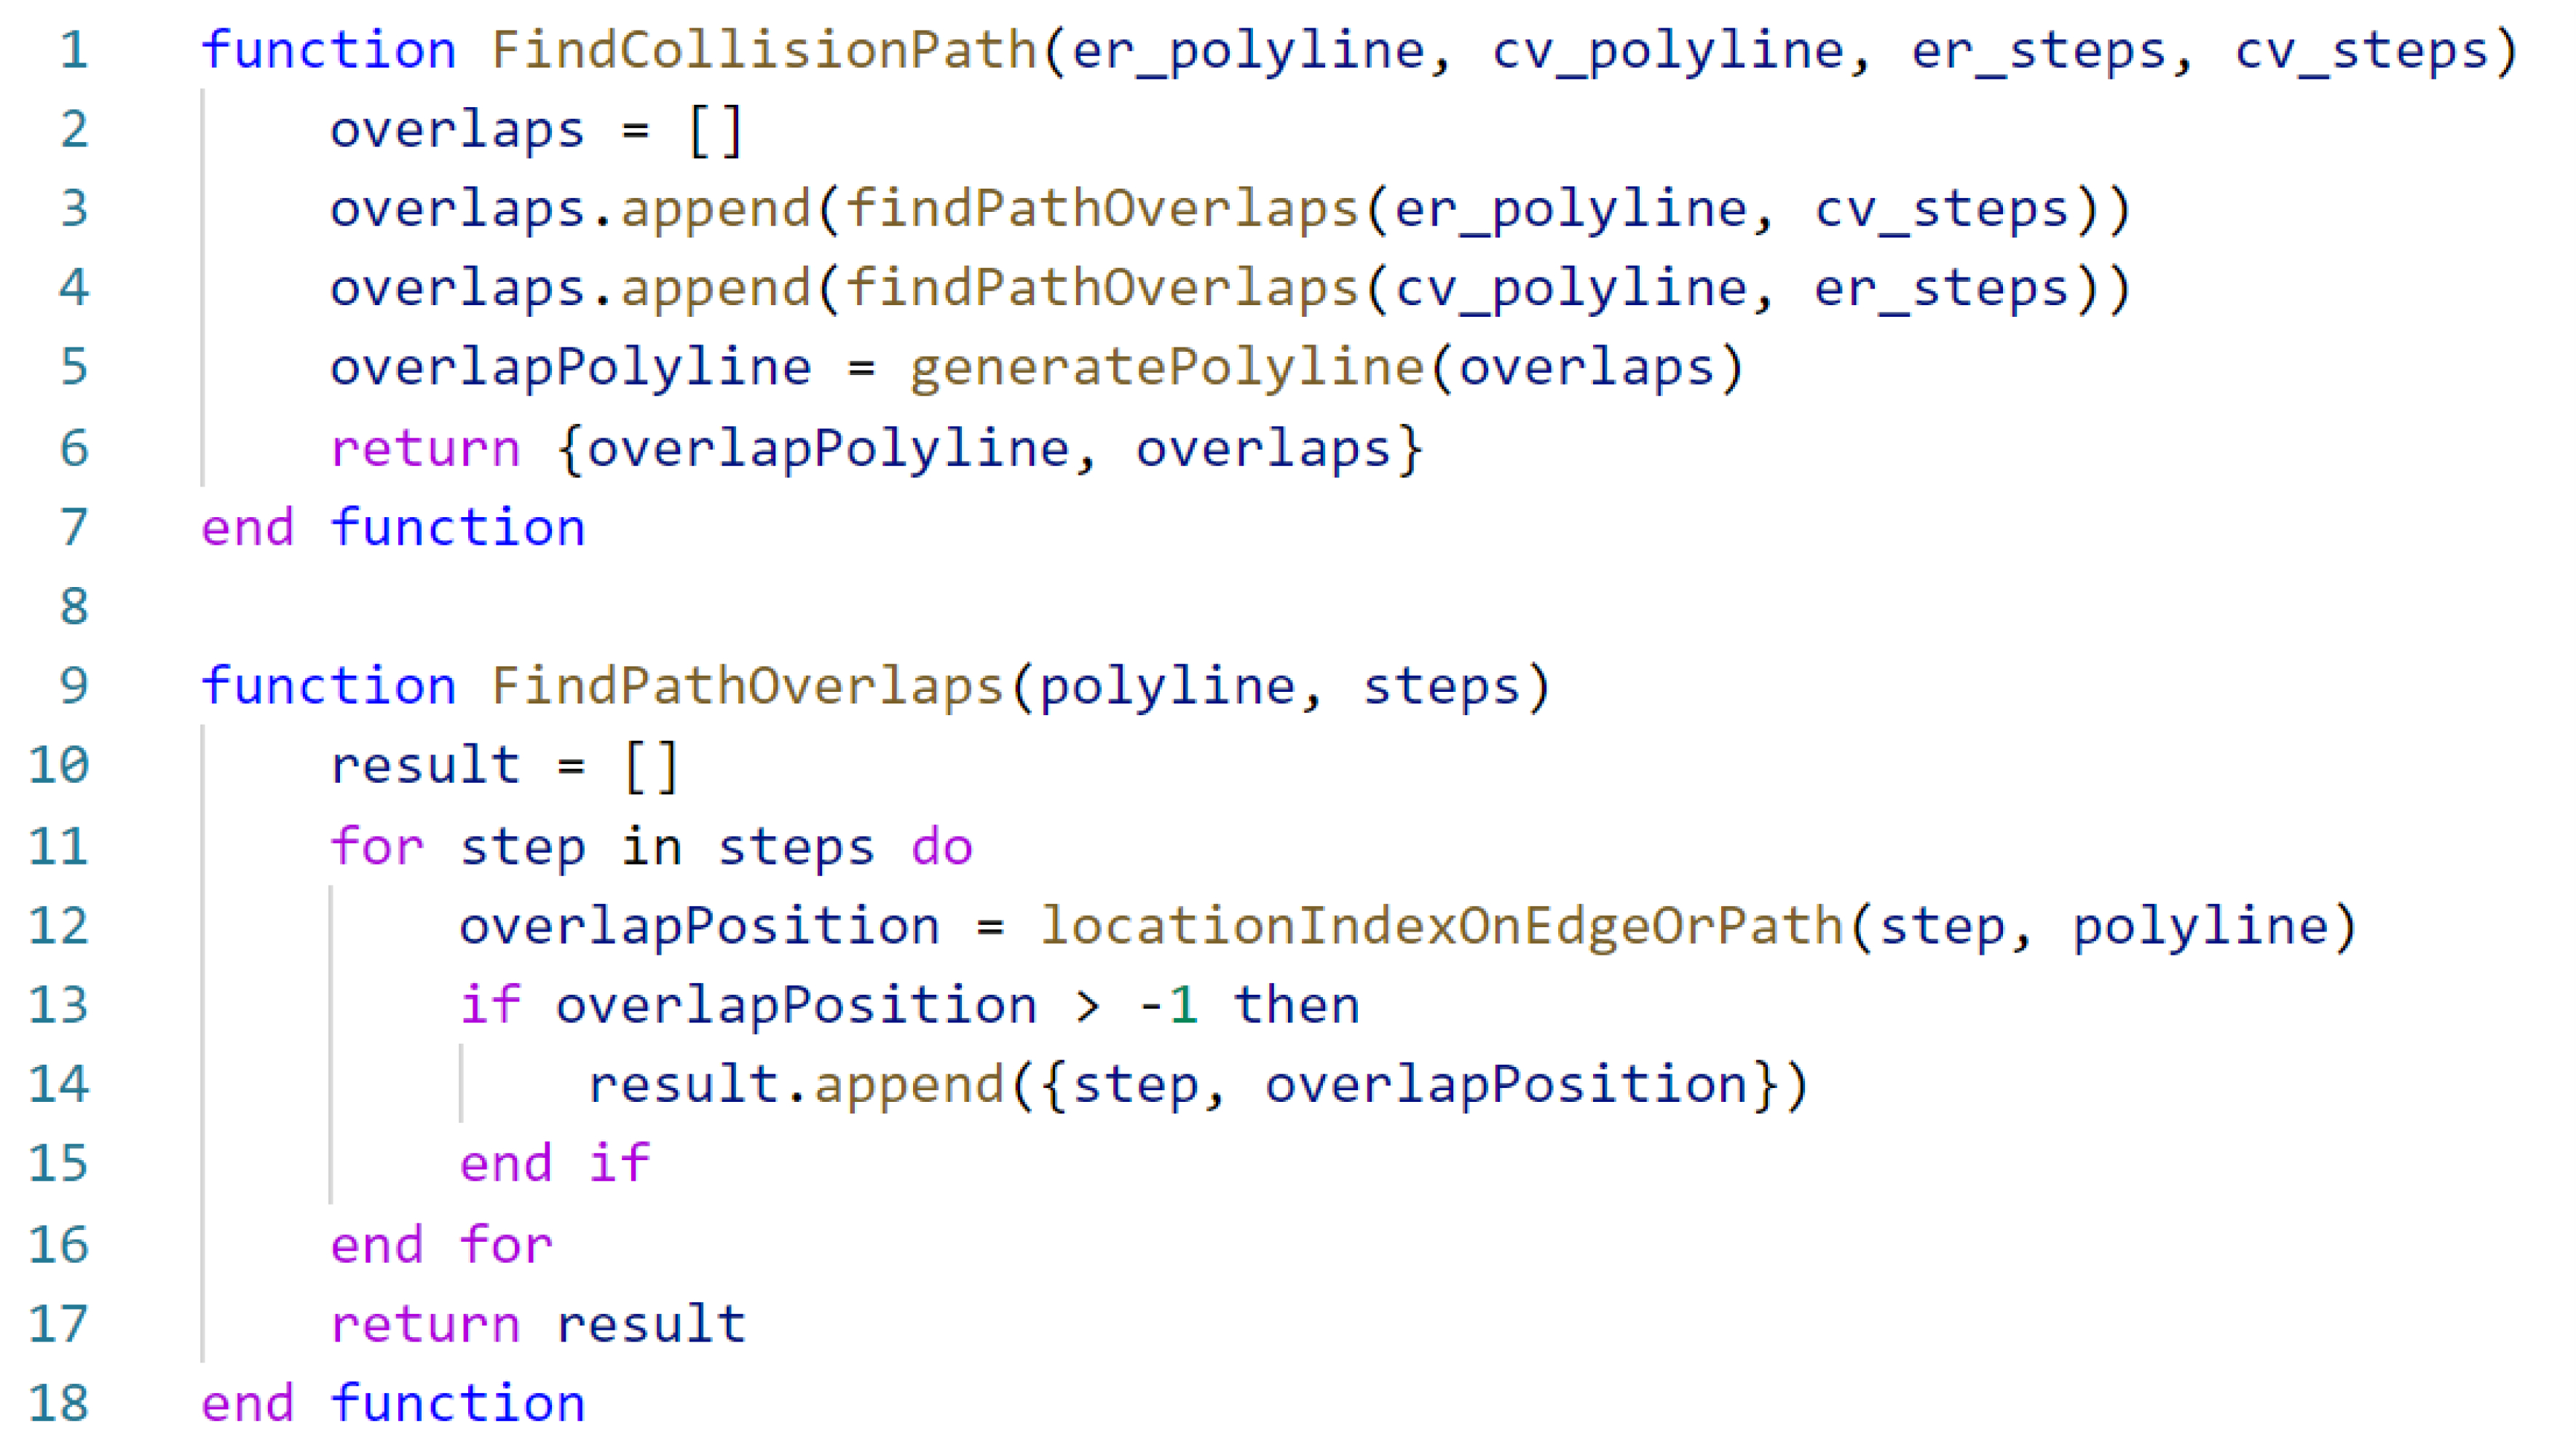
\includegraphics[width=\linewidth]{algorithm_01_psuedocode}
\caption{Pseudocode for path collision detection between the routes of an  and civilian vehicle.}
\label{fig:algorithm_01_psuedocode}
\end{figure}

![algorithm_01_diagram.jpg](https://s3-us-west-2.amazonaws.com/secure.notion-static.com/a053c2b7-eb03-450c-a037-6335e80cc406/algorithm_01_diagram.jpg)

Figure: algorithm_01_diagram

\\begin{figure}
\\includegraphics[width=\\linewidth]{algorithm_01_diagram}
\\caption{Illustration of the path collision detection algorithm between the routes of an  and civilian vehicle.}
\\label{fig:algorithm_01_diagram}
\\end{figure}

\subsection{Path Modification}

If the above process predicts a likely collision, this process is responsible for modifying the connected civilian vehicle's path to avoid roads where it predicts the collision. Figure ~\ref{fig:algorithm_02_psuedocode} and Figure ~\ref{fig:algorithm_02_diagram} describes using the time-to-collision equation as a benchmark for comparing arrival times for both vehicles and deciding where the optimal path modification should occur.

![algorithm_02_psuedocode.jpg](https://s3-us-west-2.amazonaws.com/secure.notion-static.com/91370b56-a8c9-4ace-8fbd-9a5582546e4a/algorithm_02_psuedocode.jpg)

Figure: algorithm_02_psuedocode

\begin{figure}
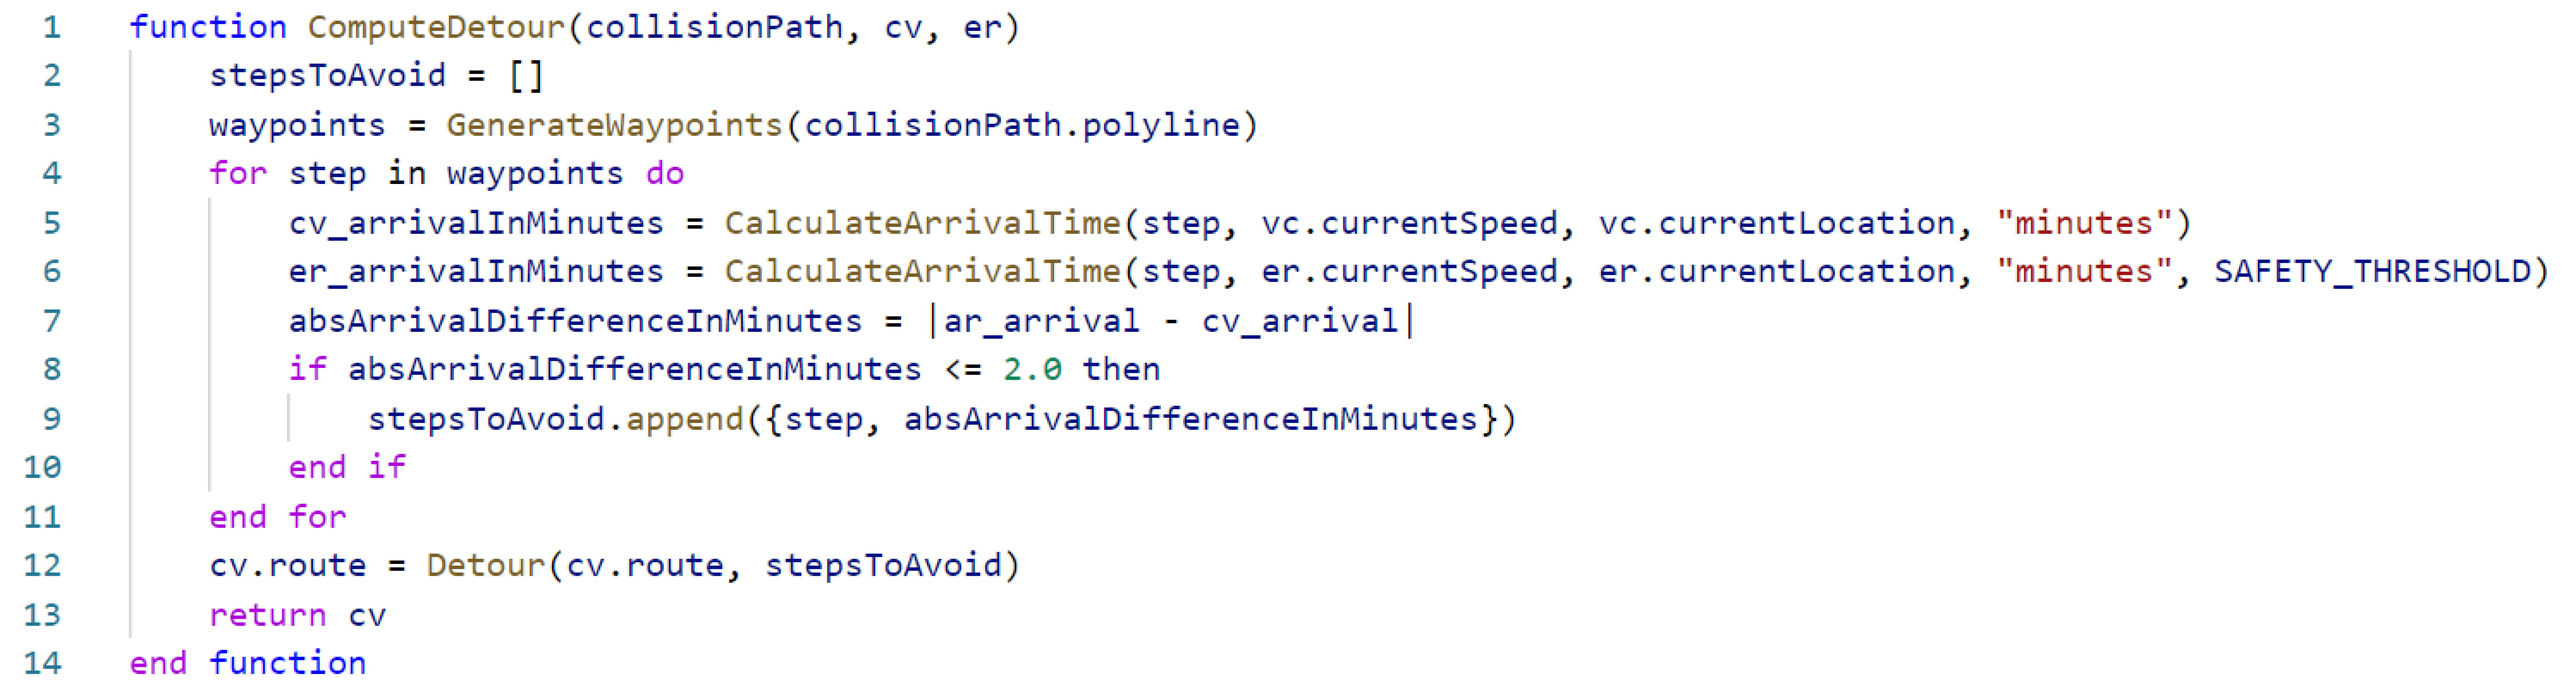
\includegraphics[width=\linewidth]{algorithm_02_psuedocode}
\caption{Pseudocode for collision avoidance algorithm.}
\label{fig:algorithm_02_psuedocode}
\end{figure}

![algorithm_02_diagram.jpg](https://s3-us-west-2.amazonaws.com/secure.notion-static.com/df47608e-e5ba-4519-b463-a236829175c6/algorithm_02_diagram.jpg)

Figure: algorithm_02_diagram

\begin{figure}
\includegraphics[width=\linewidth]{algorithm_02_diagram}
\caption{Illustration of the collision avoidance algorithm.}
\label{fig:algorithm_02_diagram}
\end{figure}

Figure ~\ref{fig:ER_heatmap} depicts an example situation where a connected \acrshort{EV}'s path overlays high traffic volume roads (section a) and how this process evenly displaces localized traffic along non-primary roads (section B). Notice that the roads overlaying the \acrshort{EV}'s path (denoted with a dotted black line) change from a red colour (high traffic volume) to a green colour (low traffic volume).

![ER_heatmap.jpeg](https://s3-us-west-2.amazonaws.com/secure.notion-static.com/a8ca5d17-3adf-4631-ab52-328a8cec7832/ER_heatmap.jpeg)

Figure: ER_heatmap

\begin{figure}
\includegraphics[width=\linewidth]{ER_heatmap}
\caption{A visual representation of the difference in traffic volume before (b) and after (b) the path modification process was applied.}
\label{fig:ER_heatmap}
\end{figure}

\section{Comprehensive Experiment Framework}

The law states that all civilian drivers must adhere to proper protocol when nearby an \acrshort{EV}, such as slowing down, moving over, and halting until the \acrshort{EV} is at a safe distance (i.e., 150 meters away) \cite{MoveOver_2021, MTO_2020}. Our \acrshort{ITS} system helps connected civilian vehicles identify \acrshort{EV} sooner, with greater context, and helps avoid route collisions. At the start of every experiment, as also done in \cite{Rizvi2007, Bahaaldin2017}, we allow the simulation to run for a consistent but arbitrary amount of time (e.g., 2 minutes), allowing the default background traffic to distribute evenly throughout the road segment. As illustrated in Figure ~\ref{fig:traffic}, we expect the primary roads to have significantly higher traffic volume (shown in red) than secondary roads (shown in green). After the calibration period, the average speeds, accelerations, and flow should level out should be constant, at which time we can apply any event or variable changes for this experiment, and we will observe and record their effects on the \acrshort{EV} arrival times.

![traffic.jpg](https://s3-us-west-2.amazonaws.com/secure.notion-static.com/54f63780-fcef-4b2d-8b95-8080e910af30/traffic.jpg)

Figure: traffic

\begin{figure}
\includegraphics[width=\linewidth]{traffic}
\caption{Stabilized traffic flow and volume of a road segment.}
\label{fig:traffic}
\end{figure}

Each experiment tests how road safety and arrival times are affected by variables such as, but not limited to, the penetration rates of connected vehicles, the number of connected and ordinary \acrshort{EV}, the number of total vehicles, and origin and destination of \acrshort{EV}. Figure ~\ref{fig:locations} does not accurately depict an actual road segment or how location points are placed. It serves to simplify the demonstration of the underlying representation of each experiment.

![locations.jpg](https://s3-us-west-2.amazonaws.com/secure.notion-static.com/e41d73d9-bddd-4b47-9da6-f9572fa8a9ee/locations.jpg)

Figure: locations

\begin{figure}
\includegraphics[width=\linewidth]{locations}
\caption{Example location of a road segment.}
\label{fig:locations}
\end{figure}

**Experiment 1:**
Have the \acrshort{EV} start in point A and travel to point C.
This route represents a firetruck commuting from outside and through an urban road segment.

**Experiment 2:**
Have the \acrshort{EV} start in point A and travel to point E, and after 2-minutes, return to corner A.
This route represents an ambulance commuting outside and stopping within an urban road segment to retrieve a patient and return to the hospital outside the road segment.

**Experiment 3:**
Have the \acrshort{EV} start at point E and travel to point A.
This route represents a police vehicle parked within a road segment responding to a call outside.

**Experiment 4:**
Have the \acrshort{EV} start at point E, travel to point F, point A, and point C.
This situation represents a police vehicle car chase, starting within the road segment.

\section{Data Analysis Methods}

Calculating traffic safety risk is a complex and ambiguous task. The authors of the \cite{leur_sayed_2002} developed a road safety risk index (RSRI), enabling a quantitative approach for measuring road safety. The RSRI is based on three isolated fundamental elements such as exposure, probability, and consequence.

\(( \text{RSRI} = \text{Exposure} \times \text{Probability} \times \text{Consequence} )\)

Where:
\begin{enumerate}
\item \textbf{Exposure} = measure to quantify the exposure of road users to potential roadway hazards.
\item \textbf{Probability} = measure to quantify the chance of a vehicle being involved in a collision.
\item \textbf{Consequence} = measure to quantify the severity level resulting from potential collisions.
\end{enumerate}

Alongside the RSRI parameters, we also consider several traffic parameters and processes known to influence traffic safety measured by proximal indicators. These include speed and speed variance, gap-acceptance in yielding situations, time headway between vehicles in traffic streams, and traffic flow rates (including derived measures such as saturation and density). We can analyze which parameters significantly impact road safety with varying CV penetration rates by tracking these parameters over multiple road segments in different driving situations.

\subsection{Exposure}

Exposure is the measure to quantify drivers' exposure to potential roadway hazards, such as nearby vehicles. It provides a score ranging from zero to a maximum of 3.0, with a high score representing high exposure.

\(\text{Exposure}_\text{urban}=(\frac{V_{i(\text{major})} \times V_{i(\text{minor})}}{V_{\text{max}(\text{major})} \times V_{\text{max}(\text{minor})}})\times3.0\)

Where:
\being{enumerate}
\item \(V_{\text{max}(\text{major})}\) = maximum volume on the major road.
\item \(V_{\text{max}(minor)}\) = maximum volume on the minor road.
\item \(V_{i}\) = volume at the location of a specific roadway.
\end{enumerate}

\subsection{Consequence}

The Consequence metric is the amount of danger the driver can incur if an accident were to happen. It is a ratio between the posted speed and maximum posted speed of a roadway segment. Maximum posted speed can equal the posted speed, or it can be based on a larger area. It provides a score ranging from zero to a maximum of 3.0, with a high score representing high consequence.

\(\text{Consequence}=(\frac{\text{Posted Speed}_i}{\text{Posted Speed}_\text{max}})\times3.0\)

Where:
\begin{enumerate}
\item \(\text{PS}_i\) = posted speed at the location of a specific roadway.
\item \(\text{PS}_\text{max}\) = maximum posted speed.
\end{enumerate}

\subsection{Volume-to-Capacity Ratio}

Volume-to-Capacity (V/C) is the ratio of current or projected demand flow rate to the capacity of a segment. It is an indicator of how close a roadway is operating to \acrshort{its} capacity. An increase in the V/C ratio indicates longer vehicle delays and queuing.

\(\text{V/C Ratio}=\frac{\text{Demand flow rate}}{\text{Capacity}}\)

Where:
\begin{enumerate} 
\item Demand flow rate = volume of vehicles on a transportation facility (vehicles per hour per lane) for a given segment length.
\item Capacity = the maximum number of vehicles a transportation facility can handle (veh/hr/ln) for a given segment length.
\end{enumerate}

\subsection{Headway}

Headway is the time difference between successive vehicles as they pass a point or segment, measured from the same point on each vehicle, expressed in seconds per vehicle.

\(\text{Headway}=\frac{\text{Spacing (ft/veh)}}{\text{Speed (ft/sec)}}\)

\subsection{Traffic Speed}

The average speed of all vehicles passing through a point or segment. Variations in the speed of vehicles within and across lanes are important traffic safety indicators.

\(v_t=\frac{1}{n}\sum^{n}_{i=1}{v_i}\)

Where:
\begin{enumerate}
\item \(v_t\) is the time-mean speed.
\item \(v_i\) is the spot speed of \(i^{th}\) vehicle.
\item \(n\) is the number of vehicles observed.
\end{enumerate}

\section{Research Validation}

We took the following steps to defend against the uncertainty that the observed results were the result of our \acrshort{ITS} system:
\begin{itemize}
\item The use of a time seed generates simulations that are generated using time seeds. This enables reproducible situations where causative factors for the results can be validated.
\item Every experiment is run with varying levels of connected vehicle penetration rates. This is done to verify whether the obtained results in the situation were a result of the connected vehicles; increasing the number of connected vehicles should amplify the results.
\end{itemize}

## Assumptions & Limitations

\subsection{Vehicle Dimensionality}

For the sake of simplicity, we assume there are only two variations in vehicle dimensions; one per vehicle model: (1) civilian vehicles and (2) \acrshort{EV}.
The dimensional specifications for our civilian vehicles are to resemble an average sedan, defining \acrshort{its} length and width as 5.0 meters and 1.8 meters, respectfully [[https://www.dimensions.com/collection/sedans](https://www.dimensions.com/collection/sedans)] {TODO: fix reference}.
Whereas the \acrshort{EV} are to resemble firetrucks with an average length and width of 10.7 meters and 2.0 meters, respectfully [[https://www.jdpower.com/cars/shopping-guides/what-are-the-dimensions-of-firetrucks](https://www.jdpower.com/cars/shopping-guides/what-are-the-dimensions-of-firetrucks), [https://www.fama.org/wp-content/uploads/2018/01/TC009-Em-Veh-Weight-Reg-FAMA-IAFC-111122.pdf](https://www.fama.org/wp-content/uploads/2018/01/TC009-Em-Veh-Weight-Reg-FAMA-IAFC-111122.pdf)] {TODO: fix references}

\subsection{Vehicle Weight}

One limitation to our research is the absence of vehicle weight. The SUMO software does not provide a way to account for the weight of a vehicle. Vehicle weight could play a significant role in maneuverability and response times, such as the time and distance needed to come to a complete stop.

\subsection{Road Elevation}

Although SUMO supports road network elevation, and that elevation could play a role in driver performance, we felt that the inclusion of this attribute only increased the complexity. Therefore, we chose to exclude this attribute from the scope of the research.

\subsection{Human Imperfection}

Human drivers are prone to make mistakes in following a provided path due to distracted driving or unforeseeable circumstances in the real world. However, our research focuses on the effectiveness of our \acrshort{ITS} in a perfect world. To reduce the complexity of our simulations, we assume all drivers have perfect driving by setting their Sigma equal to 1 on the vehicle model.
We assume that all drivers follow their routes 100\% of the time.

\subsection{Weather and Other Road Users}

The consideration of weather conditions, pedestrians, cyclists, or other vehicle types such as public transport like trains and trams is outside this research's scope.

\section{Summary}

This chapter described the design and rationale of the simulation's setup, defined the road network designs, scenario designs, software designs, simulation setup, data collection processes, explored the validity of our research and highlighted all assumptions and limitations.